\section{Methodology}

This section describes the software programs and libraries employed throughout the development of this project, as well as the hardware used to test the application created.

\subsection{Software}

\subsubsection{PX4 autopilot}
\label{subsec:px4}
PX4\footnote{\url{https://px4.io/}} is a professional open-source autopilot flight stack developed in C++ by developers from industry and academia and supported by an active worldwide community.
It powers all kinds of vehicles, from racing and cargo drones to ground vehicles and submersibles.
The flight stack software runs on a vehicle controller or flight controller hardware.
It supports both Ready-To-Fly vehicles, custom builds made from scratch,
and many additional sensors and peripherals, such as distance and obstacle sensors, GPS, camera payloads and onboard computers.

PX4 is a core part of a broader drone platform, the Dronecode Project\footnote{\url{https://www.dronecode.org/}}, that includes the QGroundControl ground station, the Pixhawk hardware for flight controllers and the MAVSDK library for integration with companion computers, cameras and other hardware using the MAVLink protocol.
PX4 was initially designed to run on Pixhawk series controllers but can now run on Linux computers and other less specific hardware.
The software controls the vehicles through flight modes. 
Flight modes define how the autopilot responds to remote control input and how it manages vehicle movement during fully autonomous flight.
The modes provide different types or levels of autopilot assistance to the user, ranging from automation of common tasks like takeoff and landing 
to mechanisms that make it easier to regain level flight or hold the vehicle to a fixed path or position.

\subsubsection{MAVLink and MavSDK}
\label{subsec:mavlink}
MAVLink\footnote{\url{https://mavlink.io/en/}} is a lightweight messaging protocol for communicating with drones and between onboard drone components.
It follows a modern hybrid publish-subscribe and point-to-point design pattern where data streams are published as topics while configuration subprotocols,
such as the mission protocol or parameter protocol, are sent as point-to-point with retransmission.
Messages are defined within XML files.
Each XML file defines the message set supported by a particular MAVLink system.

MAVSDK\footnote{\url{https://mavsdk.mavlink.io/main/en/index.html}} is a cross-platform collection of libraries for various programming languages
to interface with MAVLink systems such as drones, cameras or ground systems.
It is primarily written in C++ with wrappers available for,
among others, Swift, Python and Java.
The Python wrapper is based on a gRPC (Google Remote Procedure Call) client communicating with the gRPC server running C++.
The libraries deliver a simple API for managing one or more vehicles, 
providing programmatic access to vehicle information and telemetry
and control over missions, movement and other operations.
The libraries can be used onboard a drone on a companion computer
or on the ground from a ground station or mobile device.


\subsubsection{QGroundControl}
\label{subsec:qgc}
QGroundControl\footnote{\url{http://qgroundcontrol.com/}} is an open-source ground control station from the Dronecode Project that provides flight control and mission planning for any MAVLink-enabled drone.
It is designed with a focus on ease of use for professional users and developers.
QGroundControl connects automatically to flight controllers running the PX4 Autopilot, both through a cabled or wireless connection, as well as to any local simulator running the PX4 flight stack.

The software enables setting up the initial configuration of a flight controller and calibrating sensors and other peripherals connected to it, editing and keeping track of modified configuration parameters and sending flight commands to the drone, like arming, takeoff and landing.
It provides a map interface to keep track of the vehicle's GPS location and select target location points for planning flight missions, where the vehicle goes through each location at the designated speed and altitude.
Figure \ref{fig:qgc-map} shows the application interface on a Windows system.

\begin{figure}
  \centering
  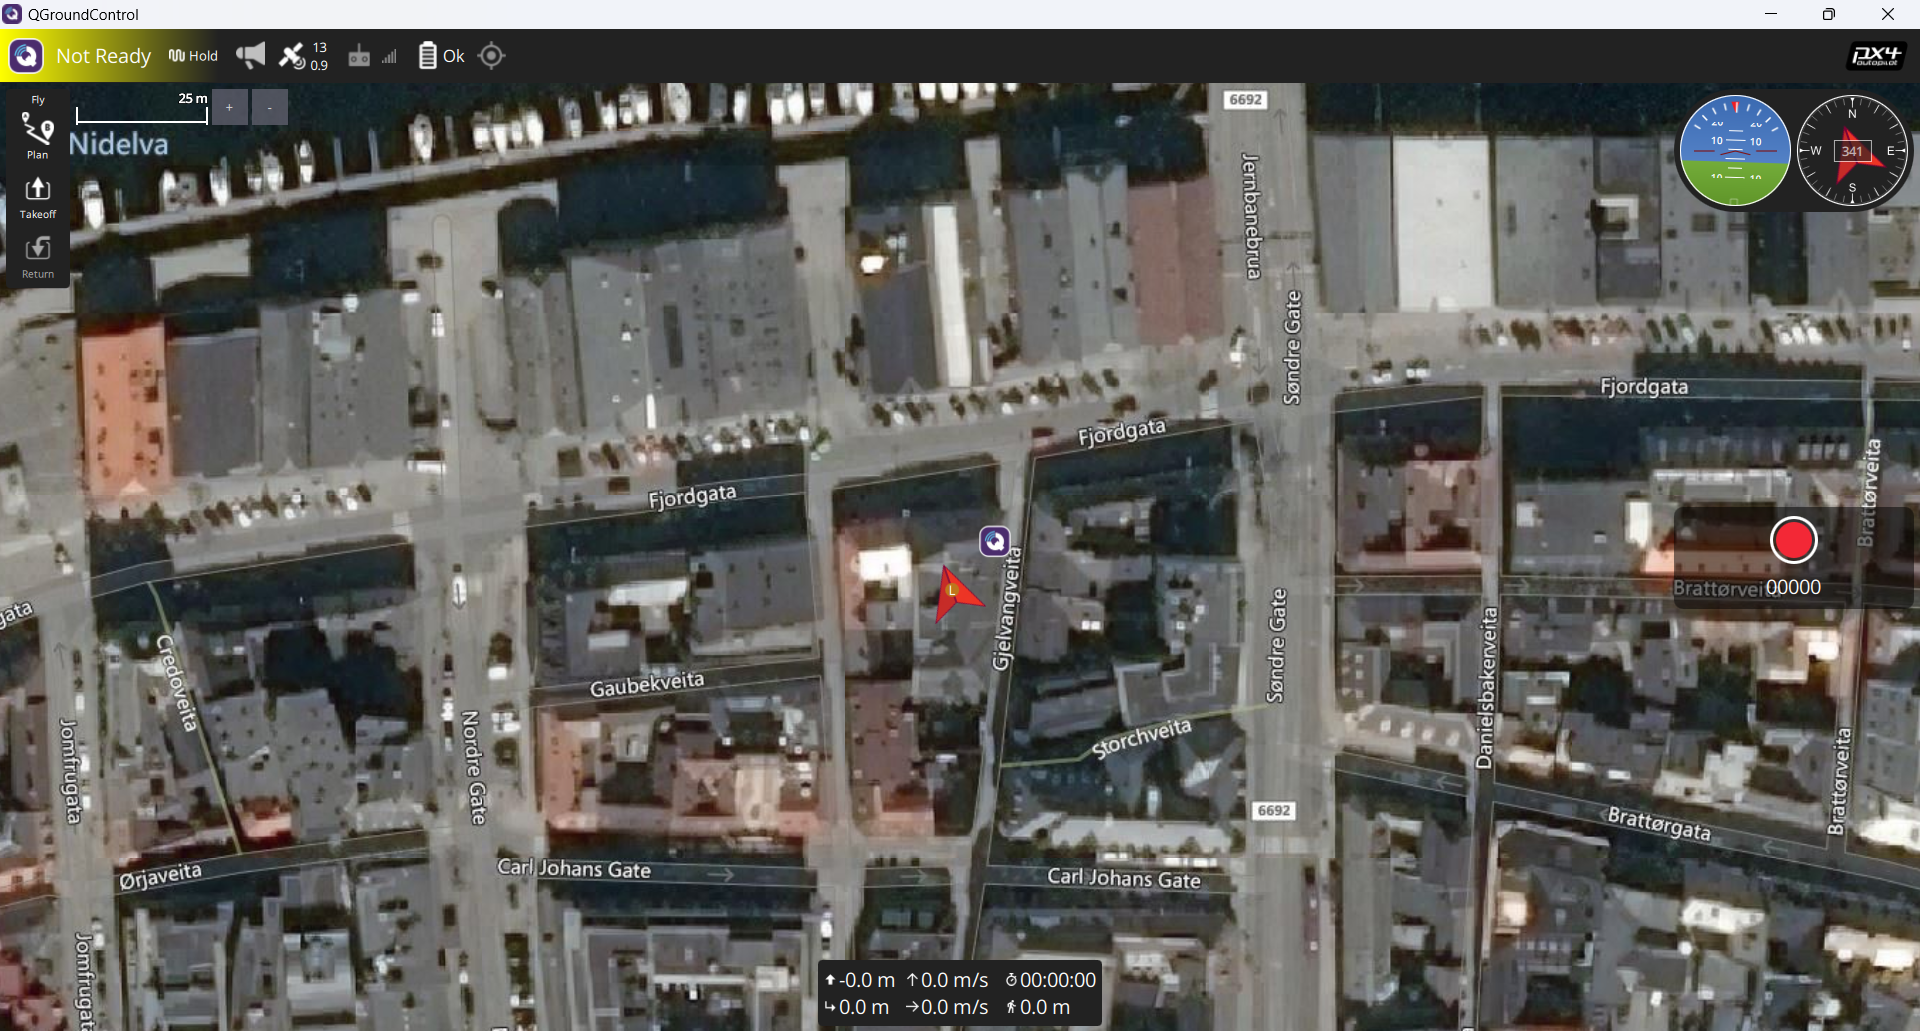
\includegraphics[width=\textwidth,keepaspectratio]{img/qgc-map.png}
  \caption{Main interface for the QGroundControl program}
  \label{fig:qgc-map}
\end{figure}

\subsubsection{Unreal Engine and AirSim}
\label{subsec:unreal}

Unreal Engine\footnote{\url{https://www.unrealengine.com/en-US}} is a 3D computer graphics creation tool best known for its game development capabilities.
It was first released in 1998 to develop first-person shooters, but its features have expanded over the years.
The engine is now used in all kinds of fields, like film and television, to create virtual sets, real-time rendering and computer-generated animation, and research, especially as a basis for virtual reality tools and developing virtual environments for the design of buildings and vehicles, among others, leveraging the engine's real-time graphic generation.
Figure \ref{fig:ue-interface} shows the program's interface when a project is loaded into the engine.

\begin{figure}
  \centering
  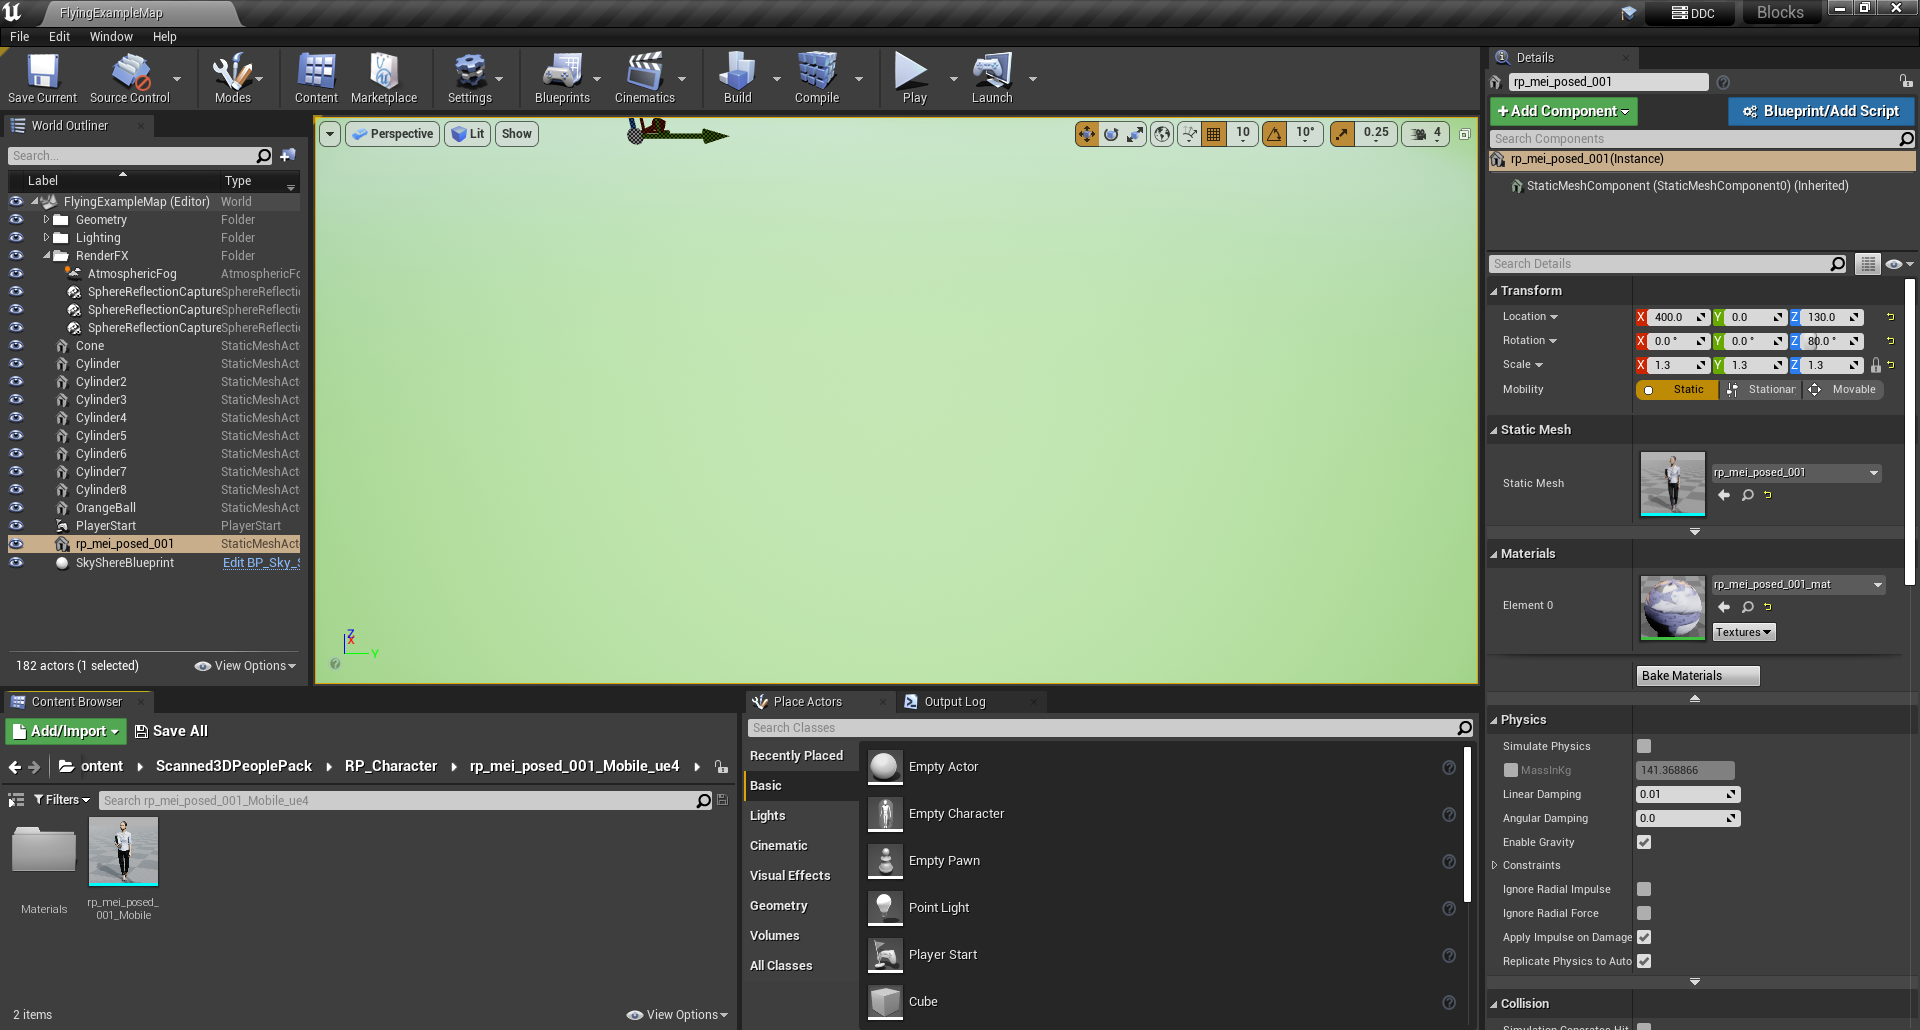
\includegraphics[width=\textwidth,keepaspectratio]{img/ue-interface.png}
  \caption{Project interface for the Unreal Engine}\label{fig:ue-interface}
\end{figure}

AirSim\footnote{\url{https://microsoft.github.io/AirSim/}} is a simulator for drones, cars and more, built on Unreal Engine and developed by Microsoft and released in 2017.
It is open-source, cross-platform, and supports software-in-the-loop (SITL) simulation with popular flight controllers such as PX4 and ArduPilot and hardware-in-the-loop (HITL) simulation with PX4 for physically and visually realistic simulations. 
It is developed as an Unreal Engine plugin that can be incorporated into any existing Unreal environment.
Its goal is to develop a platform for AI research to experiment with deep learning, computer vision and reinforcement learning algorithms for autonomous vehicles. For this purpose, AirSim also exposes APIs to retrieve data and control vehicles in a platform-independent way.
At the end of 2022, Microsoft announced that they would be releasing a new simulation platform, Project AirSim, in the coming year and subsequently archiving the original 2017 AirSim, which would stop receiving updates but remain available to the public.

\subsubsection{MediaPipe}
\label{subsec:mediapipe}
Mediapipe\footnote{\url{https://google.github.io/mediapipe/}} is an open-source project developed by Google that offers cross-platform, customizable machine-learning solutions for live and streaming media.
It supports End-to-End acceleration with built-in fast ML inference and accelerated processing even on rudimentary hardware and a unified solution that works across Android, iOS, desktop/cloud, web and IoT.
It offers a framework designed specifically for complex perception pipelines, like the real-time perception of human pose, face landmarks and hand tracking that can enable various impactful applications, such as fitness and sports analysis, gesture control and sign language recognition, augmented reality effects and more.


\subsubsection{GitHub}
\label{subsec:github}
GitHub is an online hosting service using the distributed version control system Git for software development. It is currently the most significant source code host, with over 350 million repositories.
Both the code and the front website for this project are stored in GitHub.


\subsubsection{OpenCV}
\label{subsec:opencv}
OpenCV is an open-source library for computer vision, machine learning and image processing that counts with over 2000 algorithms. 
It can be used to retrieve images or videos from cameras, extract data from them and edit them.
It is developed in C++ but offers Python wrappers that take advantage of the general-purpose programming language while maintaining the speed of the underlying computationally intensive C++ code.
OpenCV-Python employs the Numpy library, designed for highly optimized numerical operations with a syntax based on the MATLAB style.
All the OpenCV array structures are converted in Python to and from Numpy arrays. 
This makes it easy to work with other libraries that use Numpy, like Matplotlib to plot graphs.


\subsection{Hardware}
\subsubsection{Pixhawk 4}
\label{subsec:pixhawk}
The Pixhawk 4 is an advanced autopilot module designed and produced by Holybro\footnote{\url{https://shop.holybro.com/}}, a UAV parts and kits manufacturer, in collaboration with the Dronecode Project team.
It is based on the Pixhawk-project\footnote{\url{https://pixhawk.org/}} FMUv5 open hardware design, and it is optimized to run PX4 on the NuttX\footnote{\url{https://nuttx.apache.org/}} operating system by the Apache Foundation.
The Pixhawk 4 has an integrated accelerometer/gyroscope, a magnetometer, and a barometer, which enables it to drive an unmanned aerial vehicle using the PX4 flight stack natively without any other sensors.
Even so, it also includes many connector sockets to extend its features with additional sensors, input/output devices, or a companion computer.
Figure \ref{fig:pixhawk4} shows the autopilot module with all its connectors and buttons.

\begin{figure}
  \centering
  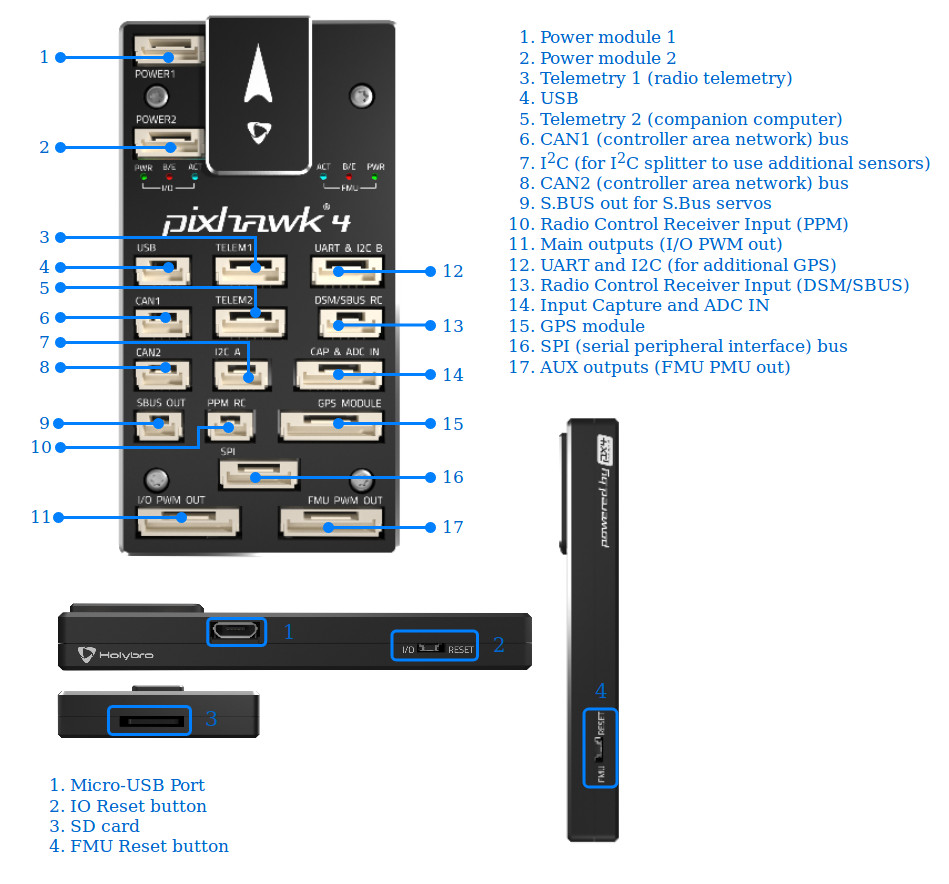
\includegraphics[width=0.6\textwidth,keepaspectratio]{img/pixhawk4.jpg}
  \caption{Side views and connector map for the Pixhawk 4 autopilot module.}
  \source{Adapted from \citetitle{px4-guide} \cite{px4-guide}.}
  \label{fig:pixhawk4}
\end{figure}


\subsubsection{Holybro X500}
\label{subsec:x500}
The Holybro X500\footnote{\url{https://docs.px4.io/main/en/frames_multicopter/holybro_x500_pixhawk4.html}} is a quadcopter designed by Holybro to use with PX4.
It comes as a ready-to-assemble development kit comprising a full carbon-fibre twill frame and the Pixhawk 4 flight controller.
The kit also includes a power management board, four motors, a GPS module, an RC receiver, and a telemetry radio.
It has a build time of approximately 3 hours and requires no specialized tools.
Figure \ref{fig:x500} shows the final result of the building process.

\begin{figure}
  \centering
  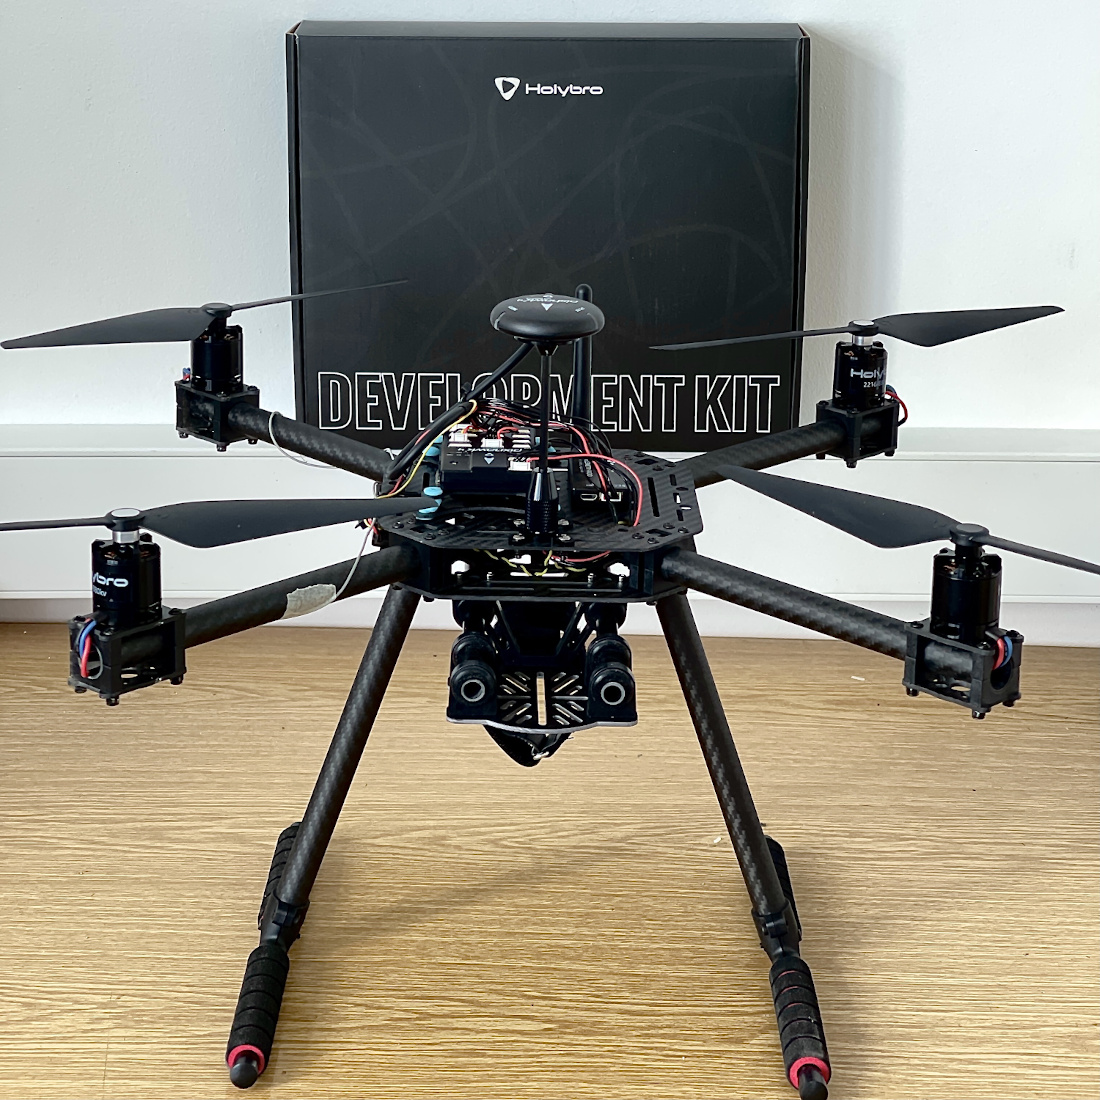
\includegraphics[width=0.7\textwidth,keepaspectratio]{img/X500-assembled.jpg}
  \caption{Fully assembled X500 kit.}
  \source{Adapted from \citetitle{px4-guide} \cite{px4-guide}.}
  \label{fig:x500}
\end{figure}

\subsubsection{Raspberry Pi 4B}
\label{subsec:rpi}
The Raspberry Pi\footnote{\url{https://www.raspberrypi.com/products/raspberry-pi-4-model-b/}} is a line of single-board computers that stands out thanks to its affordable price,
compact size, and maker-friendly design. Model 4B is an improved version of its predecessors,
significantly increasing processing power, video output, and peripheral connectivity
while maintaining the same low price and tiny size offered on past models.
This small computer comes as a bare circuit board,
without any housing or add-ons, such as a cooling fan or a power button,
but it includes USB, HDMI, and Ethernet ports and both Wi-Fi and Bluetooth connectivity,
as well as a 40-pin GPIO header, a row of input/output pins that provides direct access for connecting external devices.
The Raspberry Pi runs natively Raspbian OS, a free operating system based on Debian optimized for the Pi hardware, but it is compatible with other standard flavours of Linux.

\begin{figure}
  \centering
  \includegraphics[width=0.4\textwidth,keepaspectratio]{img/rpi4b.jpg}
  \caption{Raspberry Pi 4 Model B}
  \source{Wikimedia Commons \cite{rpi4-side}.}
  \label{fig:rpi4b}
\end{figure}
